\chapter{Sensor Data Acquisition}
In the \gls{aria} project system the air pollution sensors are connected to the Raspberry pi companion computer, which reads the data and saves it along with the telemetry data received from the autopilot. My role when I joined the \gls{aria} project was writing the necessary code to achieve this reading and saving.
Figure \ref{fig:sensor-diagram} shows a diagram of the sensors architecture.
\begin{figure}[H]
    \centering
    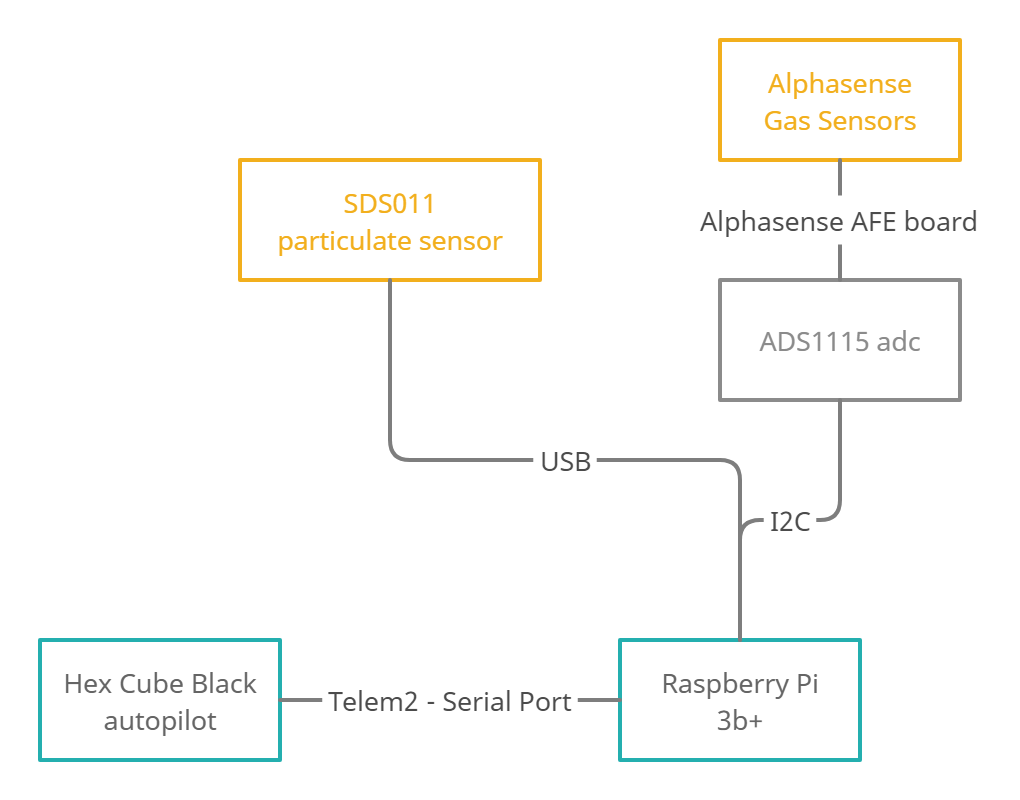
\includegraphics[width=0.7\textwidth]{images/sensor-diagram.png}
    \caption{\gls{aria} sensors architecture}
    \label{fig:sensor-diagram}
\end{figure}
The task can be divided into 2 main parts:
\begin{enumerate}
    \item Reading and saving the data from the gas and particulate sensors.
    \item Connecting the Raspberry Pi to the pixhawk autopilot and receive the telemetry data through the MAVLink protocol.
\end{enumerate}
\section{Sensor data reading and saving}
Figure \ref{fig:sensor-diagram} also shows the connections between the various components of the system. The gas sensors are connected to the Raspberry Pi via the ADS115 \gls{adc} which is in turn connected to the i2c bus on the Raspberry. The SDS011 particulate sensor is instead connected via USB.
The code to read from these sensorse was written in Python3 (from now on referred to as Python for simplicity) and uses the official Adafruit Python ADS1x15 library and a custom Python based client for the SDS011 sensor.
The script (\texttt{aria.py}), after checking the connection with the components, continuously reads the data from the sensors. In the case of the gas sensors data received from the ADS1115, the raw data is also directly processed using specific formulas which were sent to us by Alphasense (Alphasense AAN 803-05). These formulas take in input the raw electrode readings (in mV, two per gas sensor) and output the measured gas concentration (in ppb), and include a series of parameters which depend on the specific serial number of the sensor and on the external temperature. Currently the Raspberry Pi based UAV only reads data from the NO2 and CO sensors since the ADS1115 only supports 4 channels and 2 channels are required for each sensor (for the two electrodes, "AE" and "WE" in the formulas). A larger module is going to be installed in the near future.
% The formulas we use for the processing of the NO2 and CO are:
% \begin{equation}
%     NO2 = ((WE_{NO2}-WE_{eNO2})-n_NO2*(AE_{NO2}-AE_{eNO2}))/sensNO_2
% \end{equation}
% \begin{equation}
%     CO = ((WE_{CO}-WE_{eCO})-n_CO*(AE_{CO}-AE_{eCO}))/sensCO
% \end{equation}
The data is then plotted in real time using the Python pyplot library and saved to a two different csv files, one with the raw sensor data, and the other for the processed sensor data. Every row contains also the date and time, the elapsed time since the acquisition script was started and the UNIX system time which is useful to check the synchronization with the data coming from the autopilot \ref{section:telem-data}. Figure \ref{fig:cmd-and-plot} shows examples of the live plot and the csv files.
\begin{figure}[H]
    \centering
    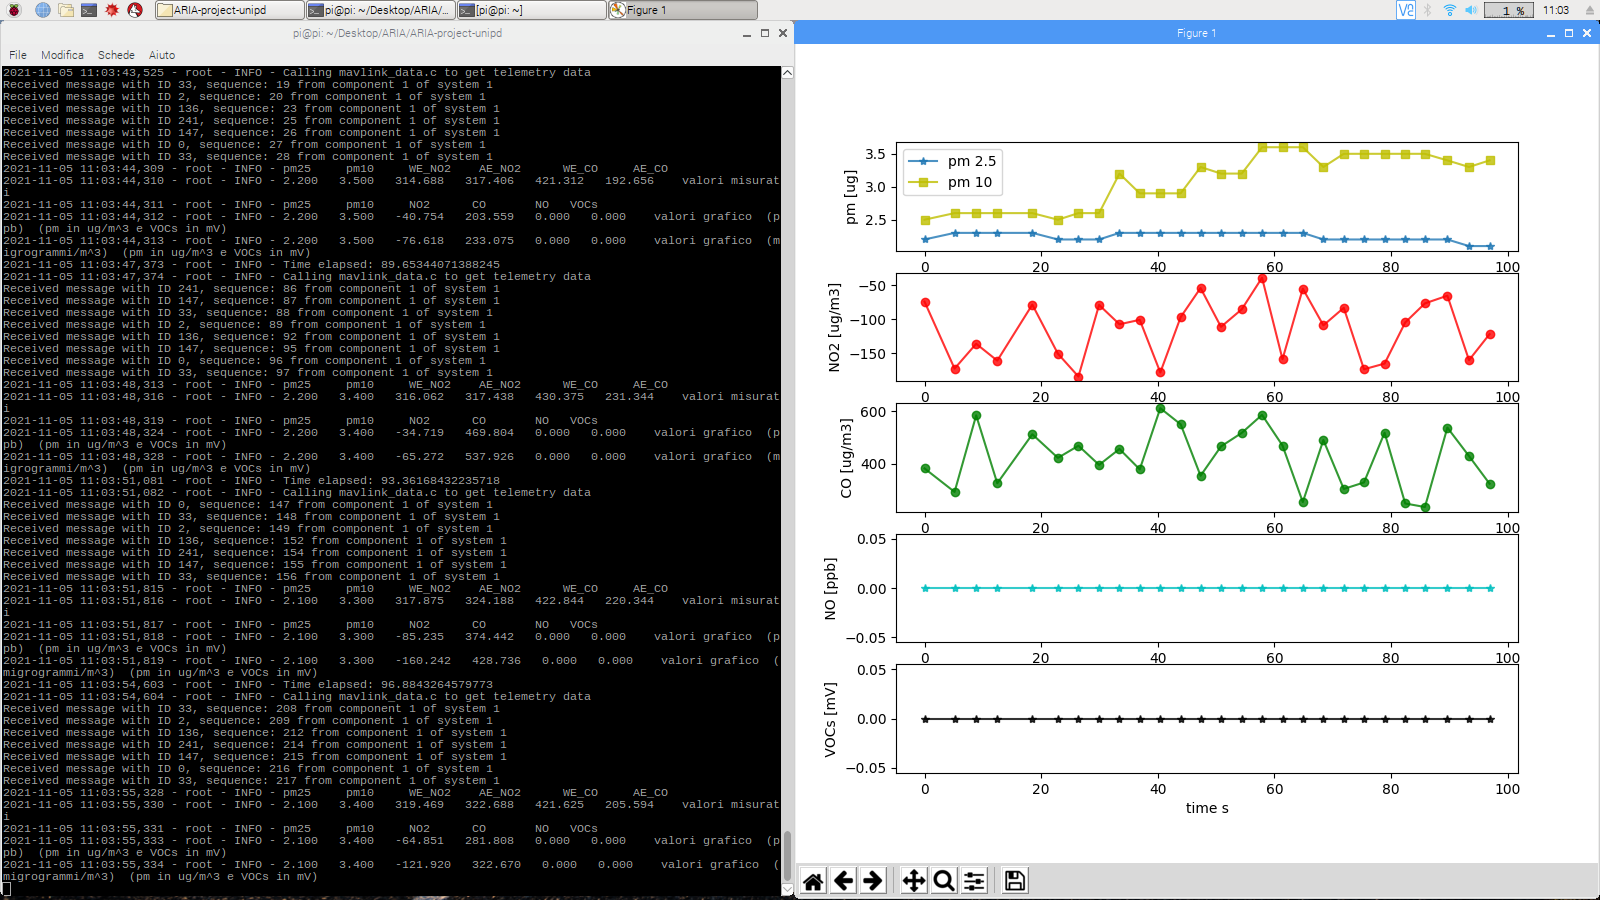
\includegraphics[width=0.8\textwidth]{images/cmd-and-plot.png}
    \caption{Screenshot of the terminal output and live plot while the script is running.}
    \label{fig:cmd-and-plot}
\end{figure}
\section{Telemetry data}
\label{section:telem-data}
To facilitate the processing of the data acquired during flight, we wanted to receive the telemetry data from the autopilot and temporally link it to the sensors data during flight. This would remove the need of a subsequent synchronization. To achieve this we connected the autopilot to the Raspberry Pi, which are both on board of the drone.
As shown in Figure \ref{fig:sensor-diagram} the Telem2 port on Hex Cube Black autopilot is connected to a serial port on the Raspberry Pi. Telem2 is the port on the Pixhawk for MAVLink communication.
\subsection{MAVLink protocol}
MAVLink is a very lightweight messaging protocol for communicating with drones and between onboard drone components. It is designed as a header-only message marshaling library.\cite{mavlink}.
\begin{figure}[H]
    \centering
    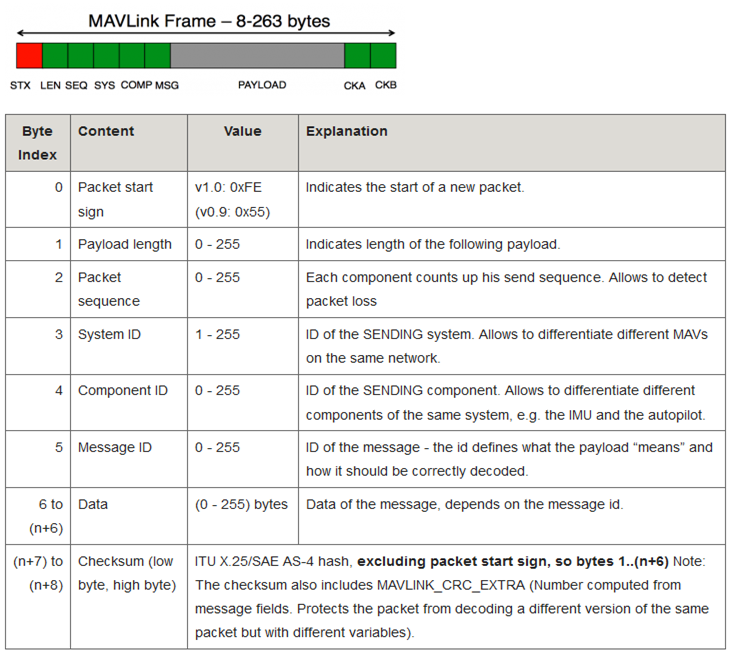
\includegraphics[width=0.7\textwidth]{images/mavlink-frame.png}
    \caption{MAVLink packet structure\cite{ardupilot}}
    \label{fig:mavlink-frame}
\end{figure}
Pixhawk and ArduPilot use MAVLink for communication. It is used between the Mission Planner \gls{gcs} software and the pixhawk, to control the UAV; and in the serial connection between the pixhawk and the Raspberry Pi companion computer, to send telemetry data.
MAVLink can transport messages and commands which are defined in a \textit{dialect}.
We used the common dialect defined in the official documentation\cite{mavlink-messages}, and the messages we needed were 'SYSTEM\_TIME' (ID \#2) and 'GLOBAL\_POSITION\_INT' (ID \#33). They, in fact, carry the UNIX time of the autopilot and telemetry data such as position, altitude and velocity. Figure \ref{fig:mavlink-messages} shows the exact content of the two messages.
\begin{figure}[H]
    \centering
    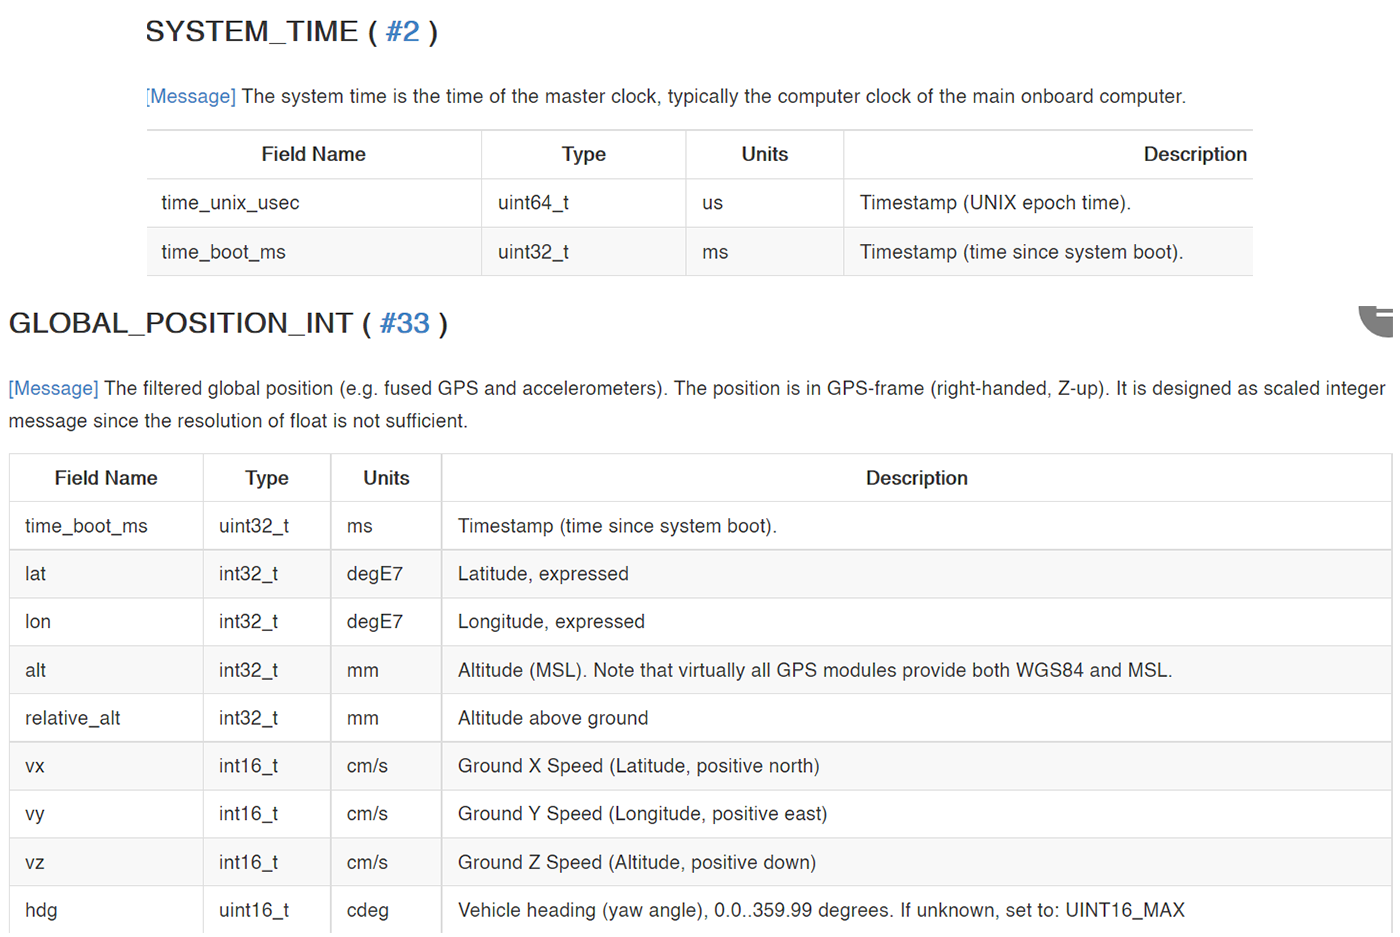
\includegraphics[width=0.8\textwidth]{images/mavlink-messages.png}
    \caption{MAVLink SYSTEM\_TIME and GLOBAL\_POSITION\_INT MAVLink messages\cite{mavlink-messages}}
    \label{fig:mavlink-messages}
\end{figure}
\subsection{Transmitting the data from the Hex Cube Black}
Firstly, through the Mission Planner, we configured the Telem2 port on the Hex Cube Black autopilot to use the MAVLink 2 protocol, as shown in Figure \ref{fig:telem2-protocol}. Serial2 is another name for the Telem2 port.
\begin{figure}[H]
    \centering
    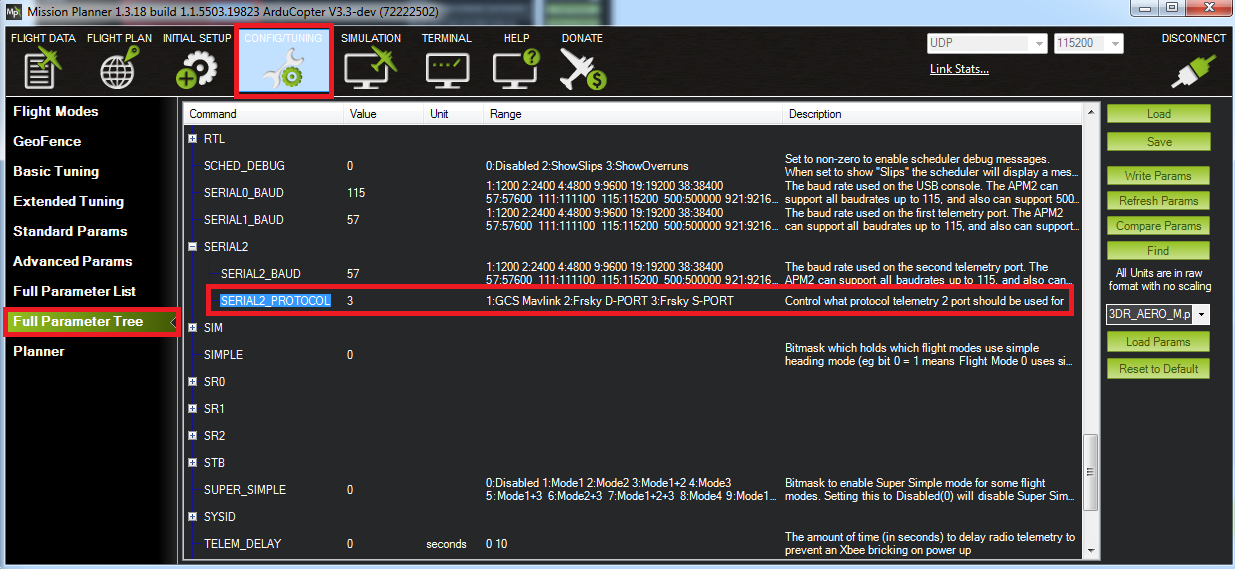
\includegraphics[width=0.8\textwidth]{images/MP-Serial2_protocol.png}
    \caption{Configuration panel in Mission Planner, highlighted is the SERIAL2\_PROTOCOL parameter\cite{ardupilot}}
    \label{fig:telem2-protocol}
\end{figure}
And we set the SERIAL2\_BAUD parameter to 9, which sets the port baudrate to 9600.

The autopilot can send the data through the Telem2 port in 2 ways:
\begin{enumerate}
    \item After receiving a REQUEST\_DATA\_STREAM MAVLink message with the ID of the requested message.
    \item By setting appropriate parameters in the autopilot to have it continuously send groups of messages through the serial connection.
\end{enumerate}
We used the second method since we always needed the same messages to be sent (SYSTEM\_TIME and GLOBAL\_POSITION\_INT) and because this approach would remove the risk of lost packages. MAVLink, in fact doesn't guarantee the reception of messages.
At \cite{ardupilot-params} can be found the list of all the ardupilot parameters. The ones we needed were the 'SR2\_EXTRA3' and the 'SR2\_POSITION'. Setting these parameters to a non zero value (possible values 0-10Hz) has the autopilot send different groups of messages. Figure \ref{fig:ardupilot-groups} shows the messages in each group.
\begin{figure}[H]
    \centering
    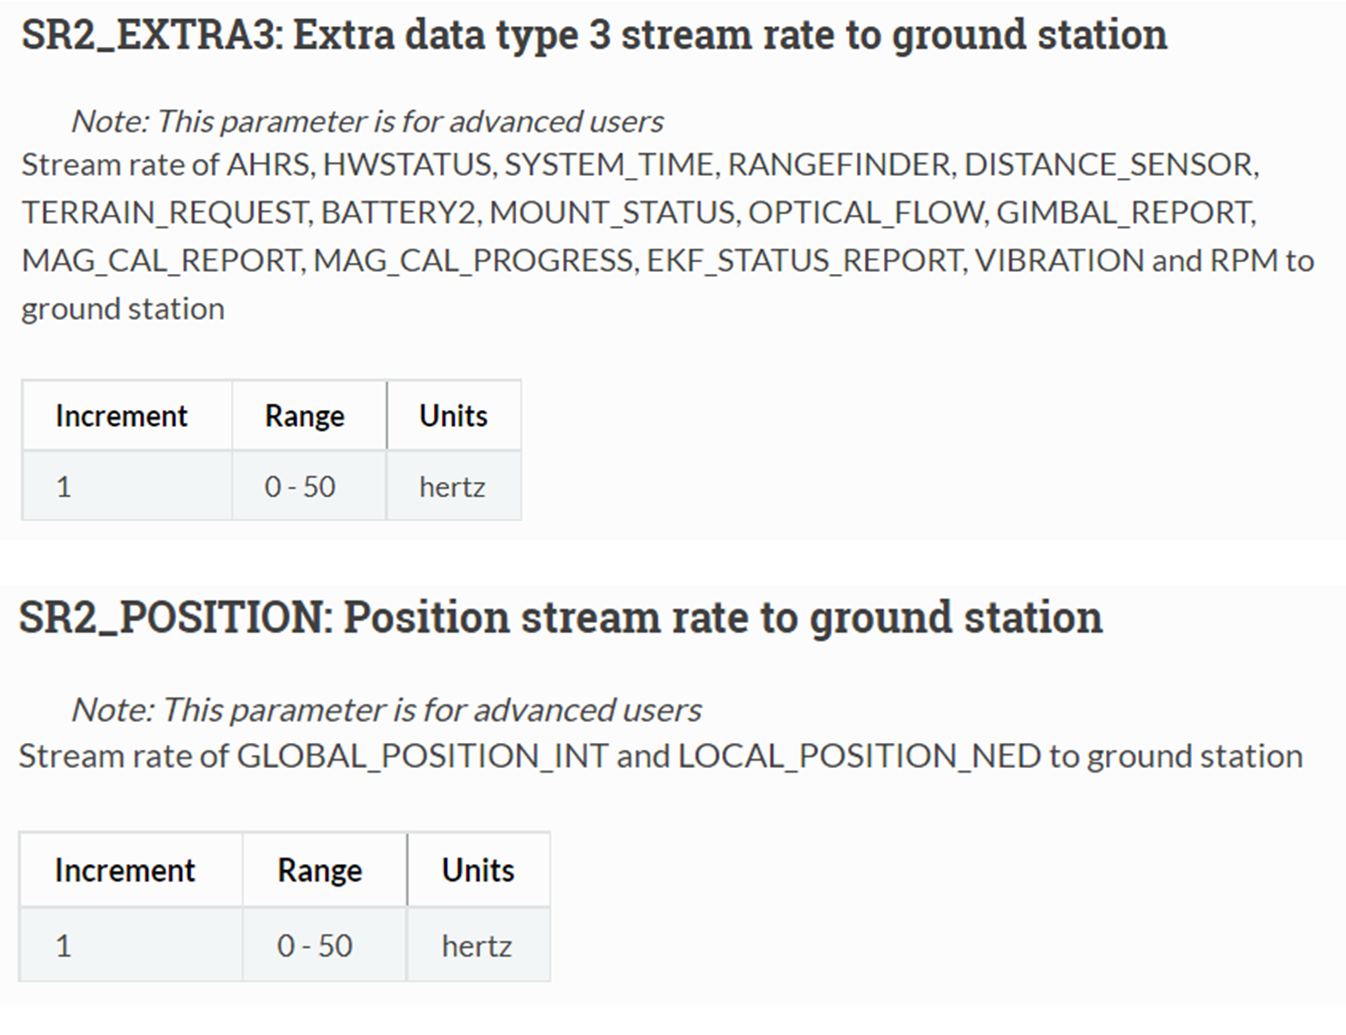
\includegraphics[width=0.8\textwidth]{images/ardupilot-groups.png}
    \caption{SR2\_EXTRA3 and SR2\_POSITION data streams from ardupilot\cite{ardupilot-params}}
    \label{fig:ardupilot-groups}
\end{figure}
Through Mission Planner we set those parameters to 2Hz.
\subsection{Receiving the data on the Raspberry Pi}
The Telem2 port on the Hex Cube Black was connected to the \gls{uart} serial port on the Raspberry Pi 3b+ on pins GPIO 15 TxD (UART) and GPIO 16 RxD (UART). The serial connections was enabled in the Raspberry via \verb|raspy-config| and was available on \verb|/dev/ttyS0|.
On the Raspberry Pi the script responsible for reading from the serial port and decoding the MAVLink messages is \verb|mavlink_data.c|. It uses the official C library for MAVLink 2, c\_library\_v2, which contains the message definitions in XML format and helper functions to decode the messages.
The code reads form the \verb|/dev/ttyS0| serial port byte by byte; parses the message with the \verb|mavlink\_parse\_char| function; checks the ID of the parsed message and if the ID is either 2 (SYSTEM\_TIME) or 33 (GLOBAL\_POSITION\_INT) saves the information in the output csv file. The following code snippet contains the reading, parsing and decoding in the case of the SYSTEM\_TIME message.
\begin{minted}{c}
    while(1) {
        if(flag)
            break;
        int n = read (fd, &byte, 1);
        if(n == -1) {
            fprintf (stderr, "error %d on read: %s", errno, portname, strerror (errno));
            return 1;
        }
        if (mavlink_parse_char(chan, byte, &msg, &status)) {
            printf("Received message with ID %d, sequence: %d from component %d of system %d\n", msg.msgid, msg.seq, msg.compid, msg.sysid);
            switch(msg.msgid) {
                case MAVLINK_MSG_ID_SYSTEM_TIME: {
                    mavlink_msg_system_time_decode(&msg, &time_message);
                    mavlink_unix_time = time_message.time_unix_usec;
                    time_since_boot = time_message.time_boot_ms;
                    flag = true;
                }   
            }
        }
    }
\end{minted}
\section{Code overview}
The code is available at this Github repository\cite{repo}.
The structure of the main script (\verb|aria.py|) is the following:
\begin{verbatim}
    Open connection with the SDS011 sensor and the ADS1115 ADC
    Call mavlink_data.c to check connection with the autopilot
    Start an infinite loop:
        Call mavlink_data.c to get telemetry data
        Acquire data from particulate and gas sensors
        Process the data
        Write data to output csv files
        Real time plot of the data with pyplot
\end{verbatim}
At every iteration of the loop both telemetry and sensors data are collected, so the rows of the csv files are time synchronized.